\documentclass{article}
\usepackage{tikz}
\usepackage{pgfplots}
\usepgfplotslibrary{fillbetween}
\begin{document}
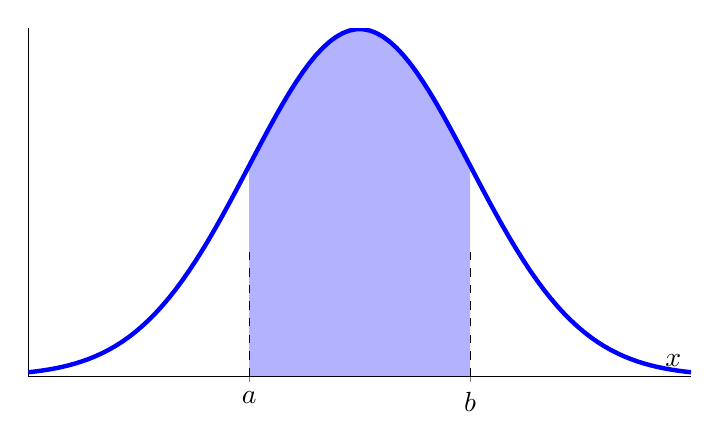
\begin{tikzpicture}
  \begin{axis}[
    axis lines=left,
    xlabel=$x$,
    xmin=-3, xmax=3,
    ymin=0, ymax=0.4,
    width=10cm,
    height=6cm,
    domain=-3:3,
    samples=100,
    every axis plot/.append style={ultra thick},
    axis x line=middle,
    axis y line=left,
    axis line style={-},
    xtick={-1,1},
    xticklabels={$a$, $b$},
    ytick=\empty,
    legend style={at={(0.9,0.9)}, anchor=north}
  ]

  \addplot [name path=curve, blue, domain=-3:3] {1/sqrt(2*pi)*exp(-x^2/2)};

  \path[name path=axis] (axis cs:-1,0) -- (axis cs:1,0);

  \addplot [blue, opacity=0.3] fill between [of=curve and axis, soft clip={domain=-1:1}];

  \draw [dashed] (axis cs:-1, 0) -- (axis cs:-1, {1/sqrt(2*pi)*exp(-1)});
  \draw [dashed] (axis cs:1, 0) -- (axis cs:1, {1/sqrt(2*pi)*exp(-1)});
  \end{axis}
\end{tikzpicture}
\end{document}
